% !TeX root = ../main.tex

\chapter{相关工作}

\section{DXT纹理格式}

DXT是一组有损的纹理压缩格式,
最初由S3 Graphics公司的Iourcha等\cite{iourcha1999system}开发,
并在20世纪90年代末被引入游戏图形领域。
它最早作为S3 Graphics的Savage 3D图形芯片的一部分推出,
随后被微软采纳并集成到DirectX 6.0及更高版本中,
目前已经成为PC平台上最主要的纹理格式。与基于离散余弦变换与熵编码的JPEG格式不同,
DXT格式采用基于块的压缩方法,将每4×4像素块存储为固定大小的数据,
从而在GPU上实现高效解码。
目前DXT格式共包含BC1至BC7共7种子格式,其中BC6用于压缩HDR纹理(浮点纹理),其余6种格式用于压缩LDR纹理(0-255的整数纹理)。
每种格式都针对特定类型的纹理设计,所有格式都将4x4的像素块转换为64位或128位的数据,从而在24位RGB图像上实现了6:1的压缩比,
在32位RGBA图像上实现了4:1的压缩比。
DXT格式仅指定用于解压缩纹理的方法,允许实施者设计适合其特定需求的压缩算法。

\subsection{BC1纹理格式}

BC1格式是DXT中最基础的块压缩格式,如图\ref{fig:BlockCompression}所示,它将未压缩的纹理数据分为4×4大小的块,
压缩每个块并分别存储数据。因此需要压缩的纹理尺寸必须是 4 的倍数。

\begin{figure}[htbp]
    \centering
    \includegraphics[width=0.75\textwidth]{figures/BlockCompression.png}
    \caption{块压缩示例(第一个块显示了标记为 a到p 的 16 个纹素)\cite{BC1-5}}
    \label{fig:BlockCompression}
\end{figure}

BC1格式仅支持RGB纹理,对Alpha通道仅存储1位Alpha值,表示纹理完全透明或完全不透明。
BC1首先将纹理划分成4x4大小的纹素块,
每个块压缩成两个16位的RGB颜色端点以及16个权重,
解压时根据每个纹素对应的权重值,线性插值两个颜色端点得到最终的颜色值。
颜色端点与权重的位数如图\ref{fig:BC1}所示,每个颜色端点使用RGB 5:6:5共16位存储,
每个纹素的权重由2位存储。最终每个4x4纹素块存储为64位,即8字节,
相较于压缩前的每纹素24位的RGB纹理共48字节达到了6:1的压缩比。

\begin{figure}[htbp]
    \centering
    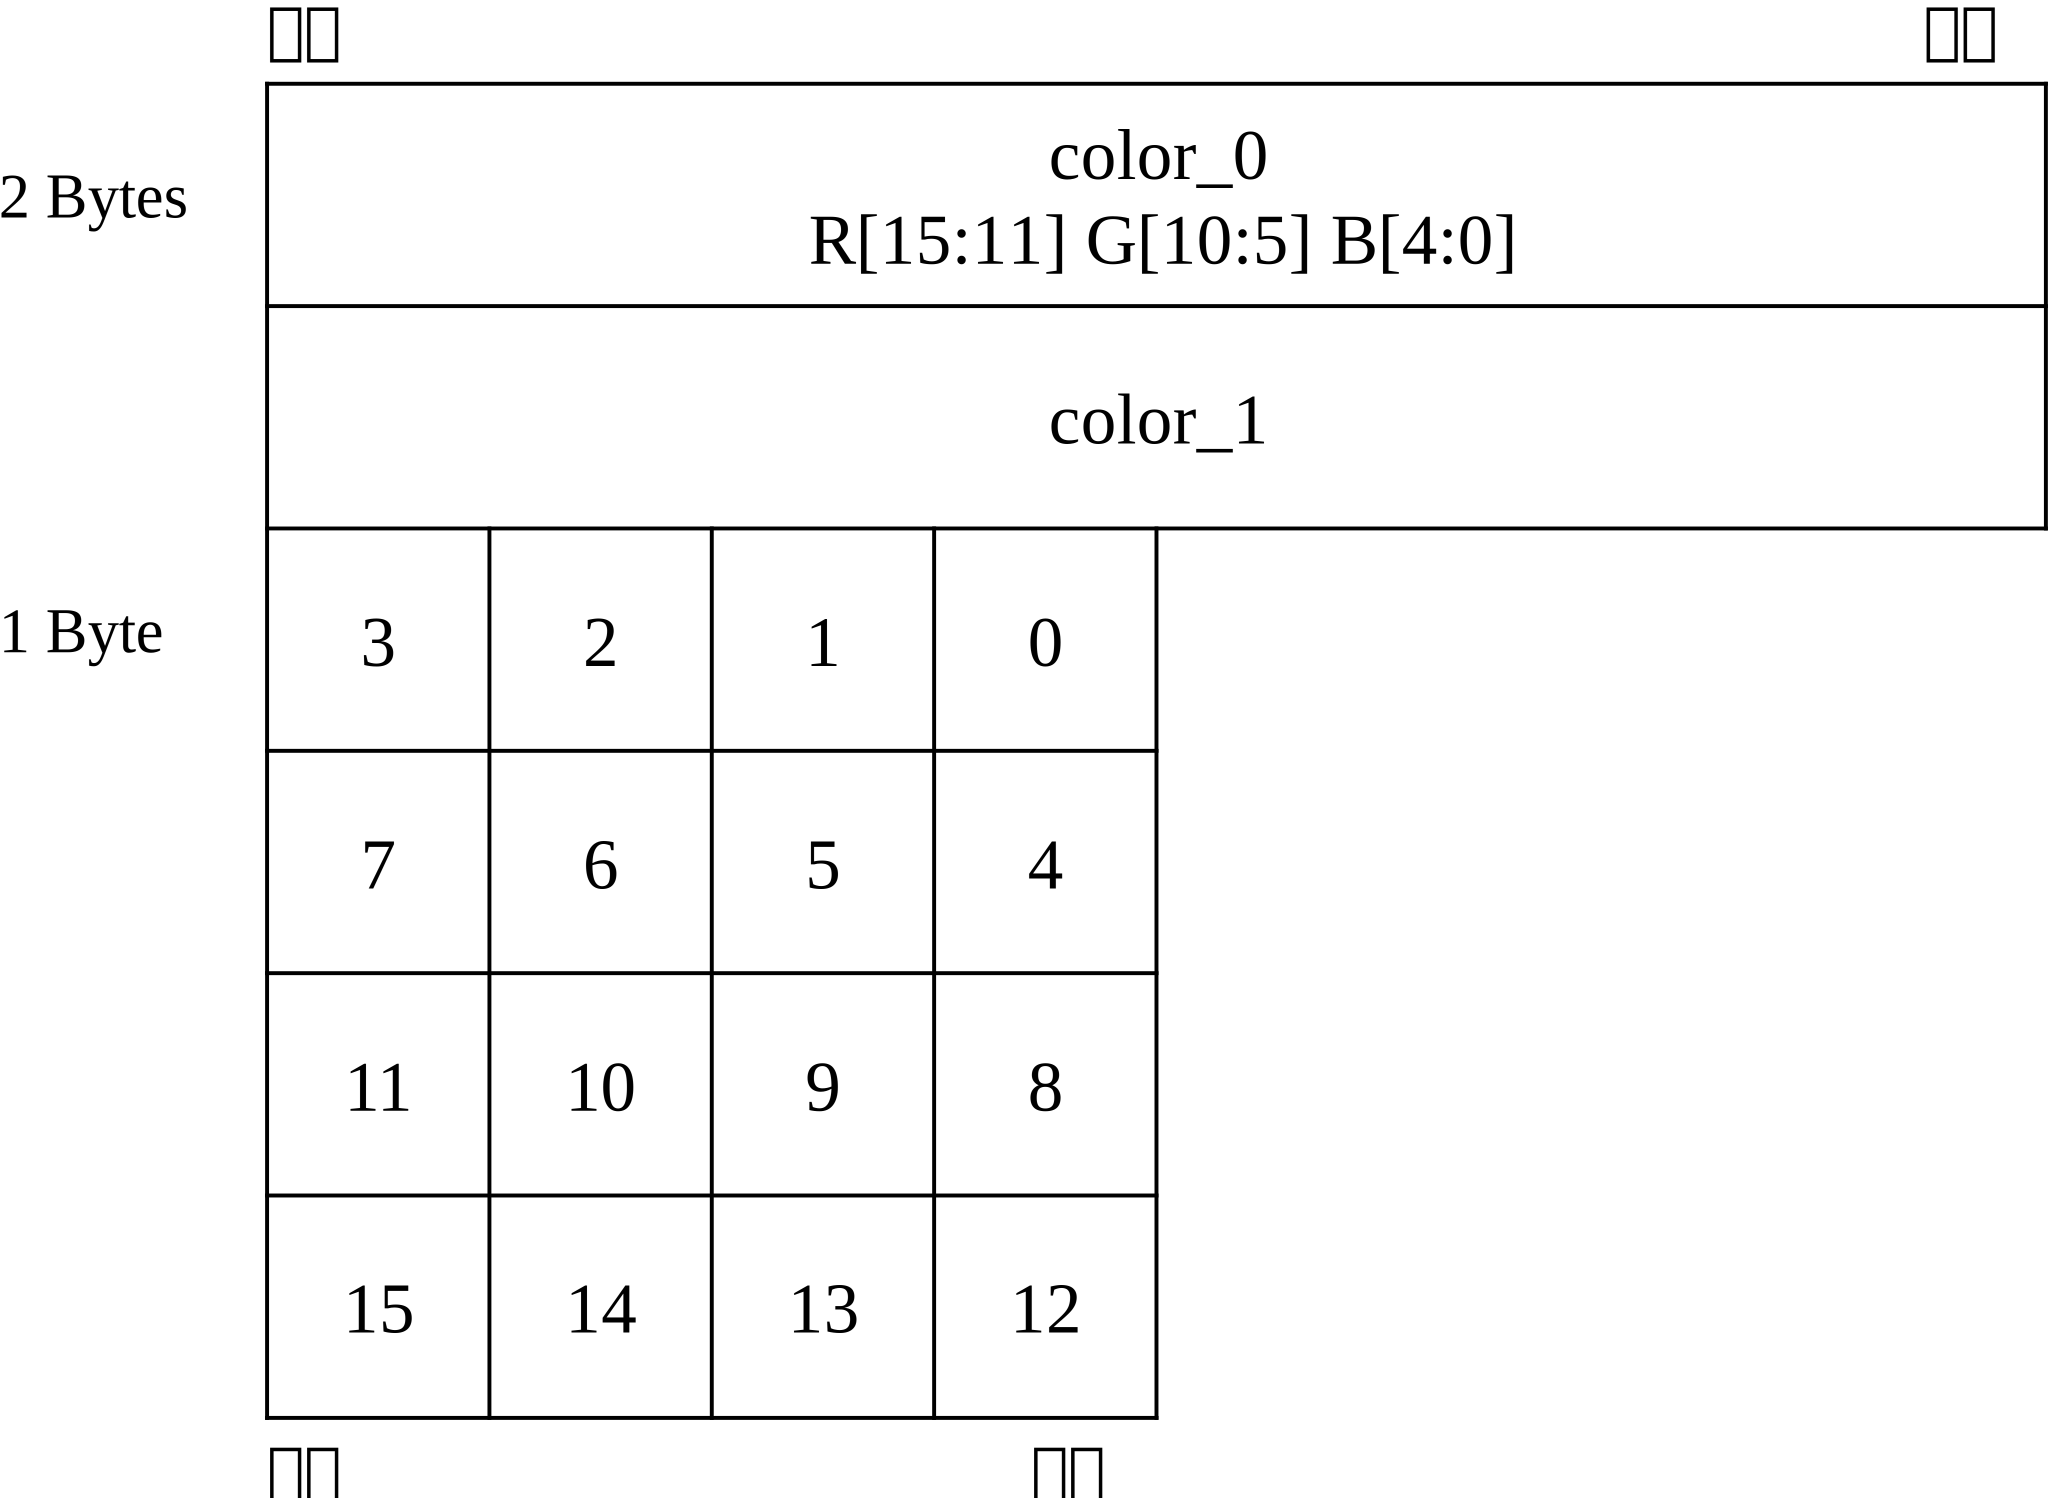
\includegraphics[width=0.75\textwidth]{figures/BC1.png}
    \caption{BC1格式中每个块的数据布局\cite{BC1-5}}
    \label{fig:BC1}
\end{figure}

BC1对颜色端点与权重的量化方式为均匀量化,除BC6外,
DXT格式中的其余6种格式都使用与BC1相同的均匀量化方式量化颜色端点与权重。
其量化函数为:
\begin{equation}\label{eqn-6}
    Q(r)=\left \lfloor r \times (2^{b}-1) \right \rceil
\end{equation}
其中$r$表示量化前的0-1浮点值(对于0-255整数范围的颜色值需要归一化到0-1之间),$b$表示量化位数,$Q(r)$表示量化后的整数值,$\lfloor \cdot \rceil$表示四舍五入函数。

解量化函数为:
\begin{equation}\label{eqn-6}
    Q'(q)=\frac{q}{2^{b}-1}
\end{equation}
其中$q$表示量化后的整数值,$b$表示量化位数,$Q'(q)$表示解量化得到的0-1浮点值,可以
通过乘255恢复原始纹理。

解压缩过程中颜色端点的线性插值过程如图\ref{fig:LinearInterpolate}所示,
权重被量化为0至1之间的浮点数后,
作为系数对颜色端点进行线性插值,分别对应了两个颜色端点构成的线段上的不同位置。
DXT格式中的所有子格式(BC1-BC7)纹理解压缩时都具有相同的颜色端点线性插值过程。

\begin{figure}[htbp]
    \centering
    \includegraphics[width=0.75\textwidth]{figures/LinearInterpolate.pdf}
    \caption{颜色端点的线性插值\cite{ASTC}}
    \label{fig:LinearInterpolate}
\end{figure}

\subsection{BC2-BC5纹理格式}
BC2格式增加了对Alpha通道的支持,如图\ref{fig:BC2}所示,在BC1的基础上将Alpha通道存储为单独的4位值,相比BC1增加了64位。
最终每个4x4纹素块存储为16字节,相较于压缩前的每纹素32位的RGBA纹理共64字节达到了4:1的压缩比。

\begin{figure}[htbp]
    \centering
    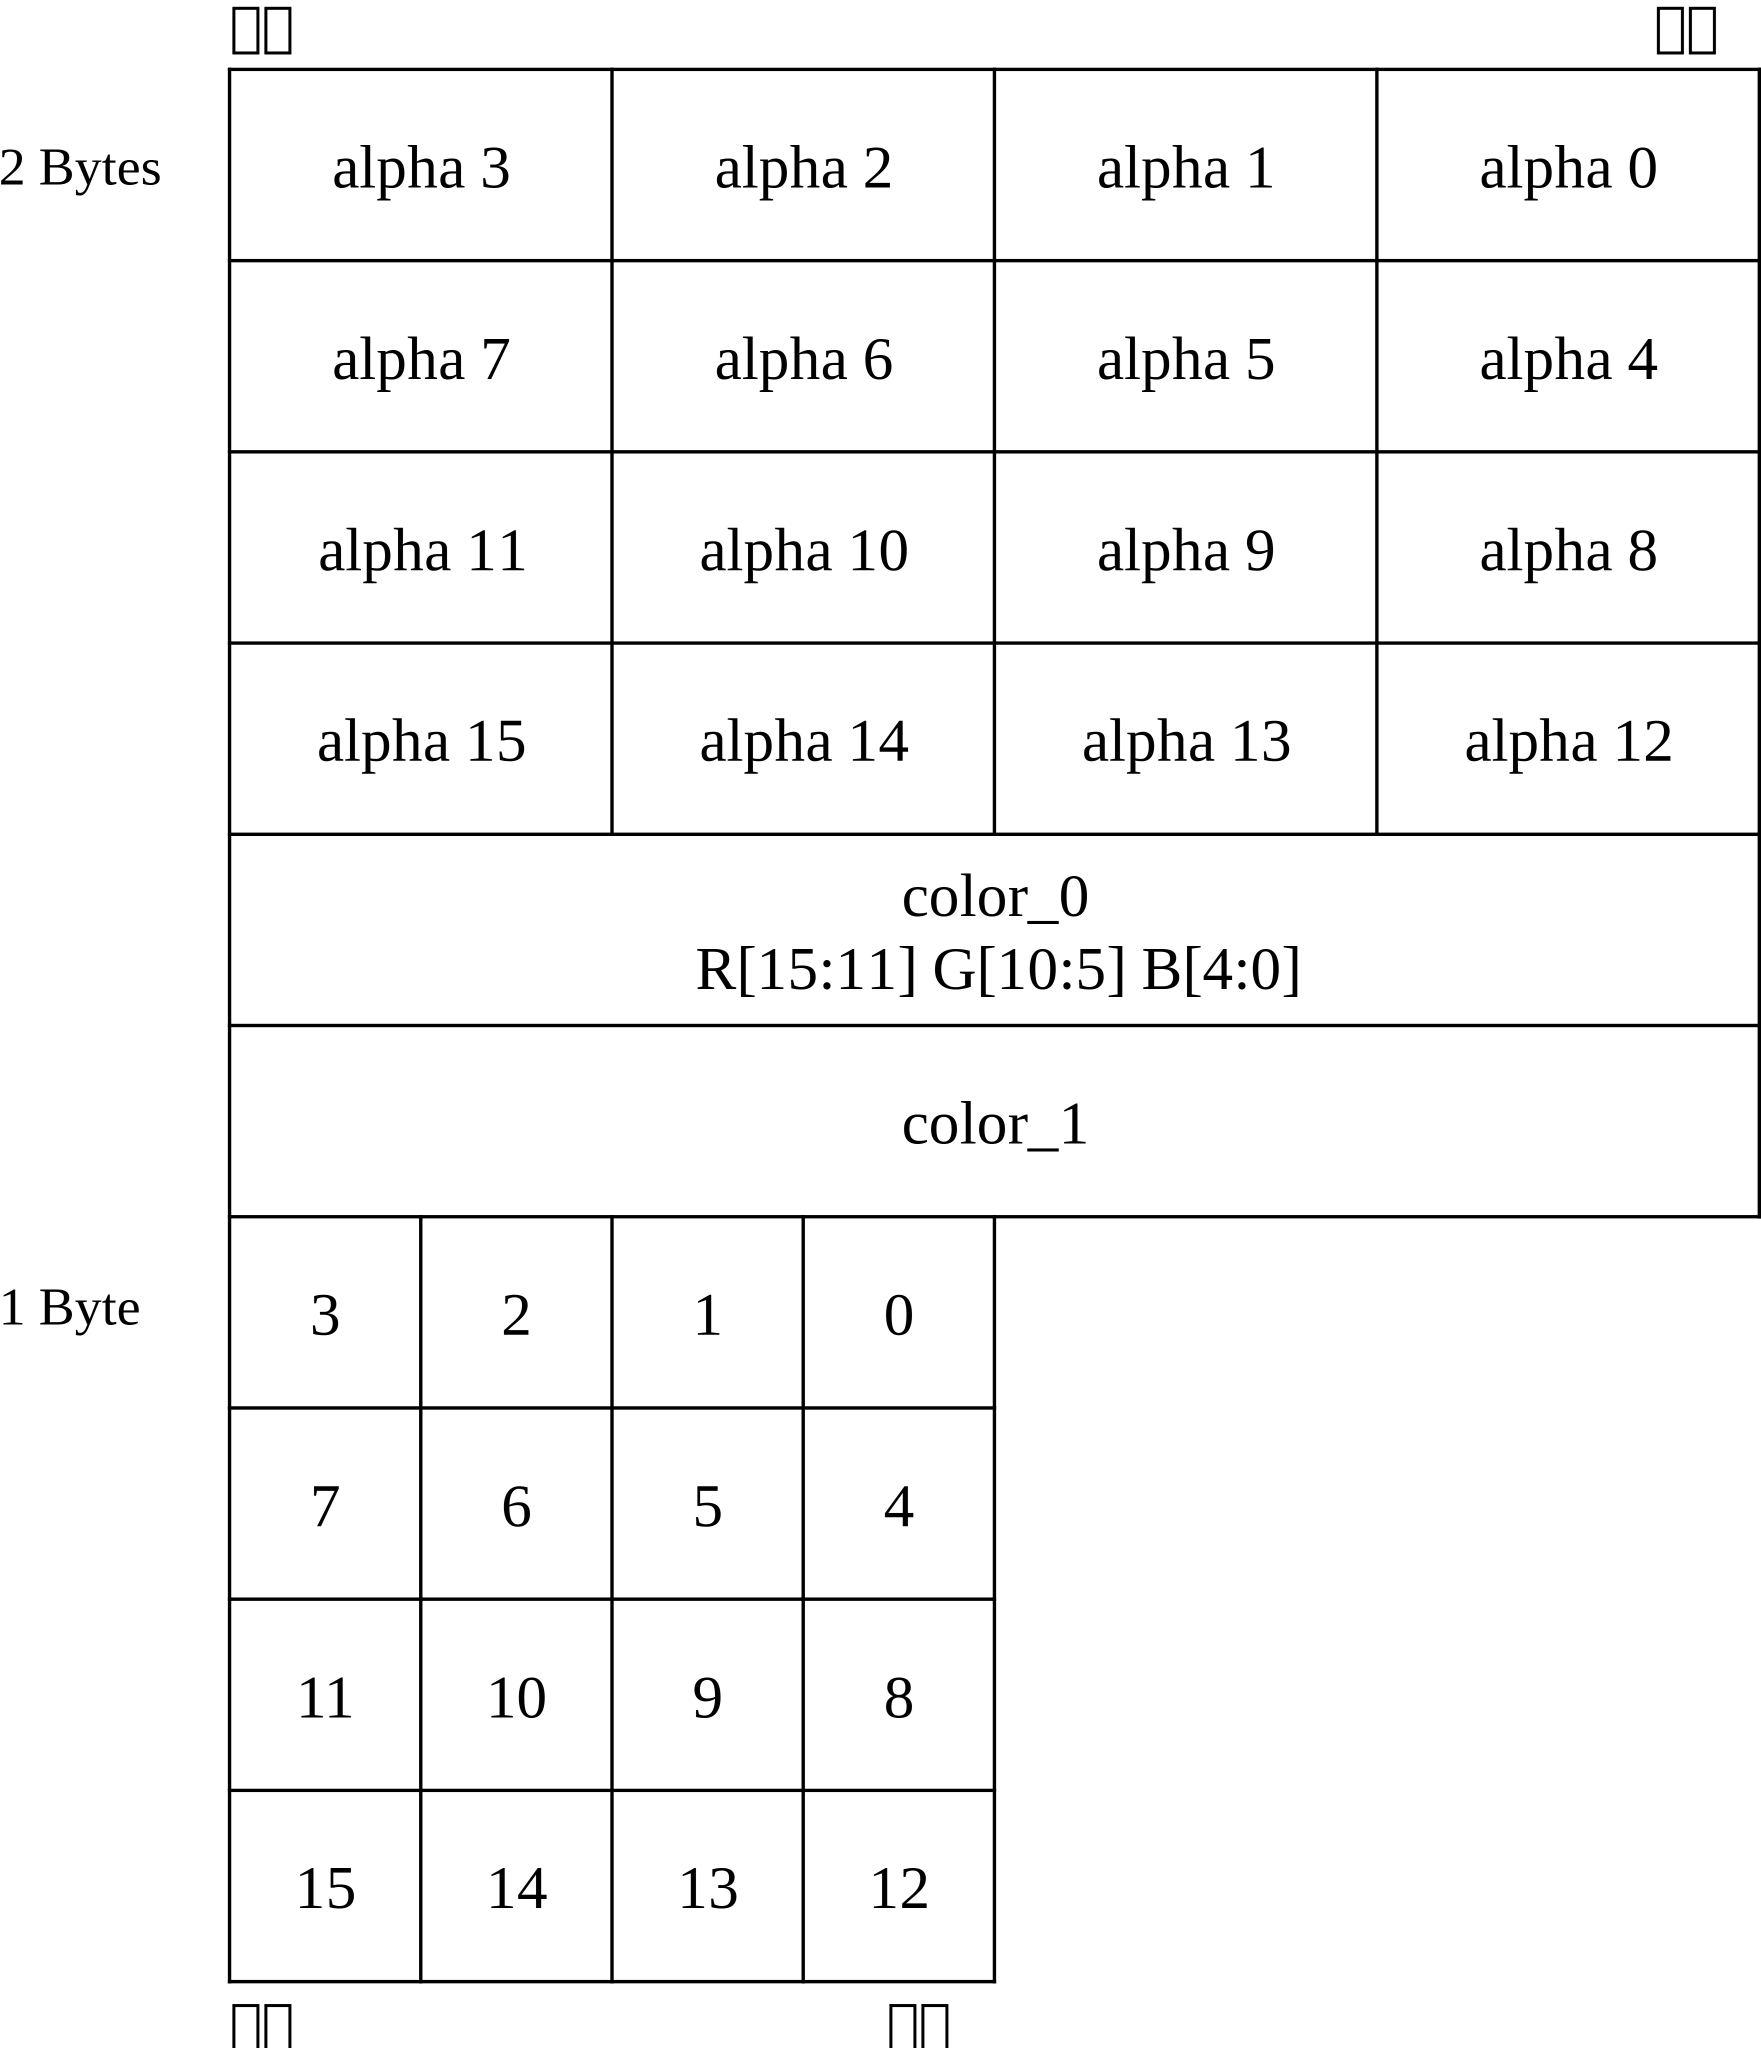
\includegraphics[width=0.7\textwidth]{figures/BC2.png}
    \caption{BC2格式中每个块的数据布局\cite{BC1-5}}
    \label{fig:BC2}
\end{figure}    

BC3格式同样支持Alpha通道,如图\ref{fig:BC3}所示,其RGB通道的存储与BC1相同,Alpha通道的存储采用了类似存储RGB通道的方式,即
存储两个8位的Alpha 端点以及16个3位的Alpha权重,解压时根据权重对两个Alpha端点进行线性插值,BC3同样相比BC1增加了64位。
最终每个4x4纹素块存储为16字节,相较于压缩前的每纹素32位的RGBA纹理共64字节达到了4:1的压缩比。

\begin{figure}[htbp]
    \centering
    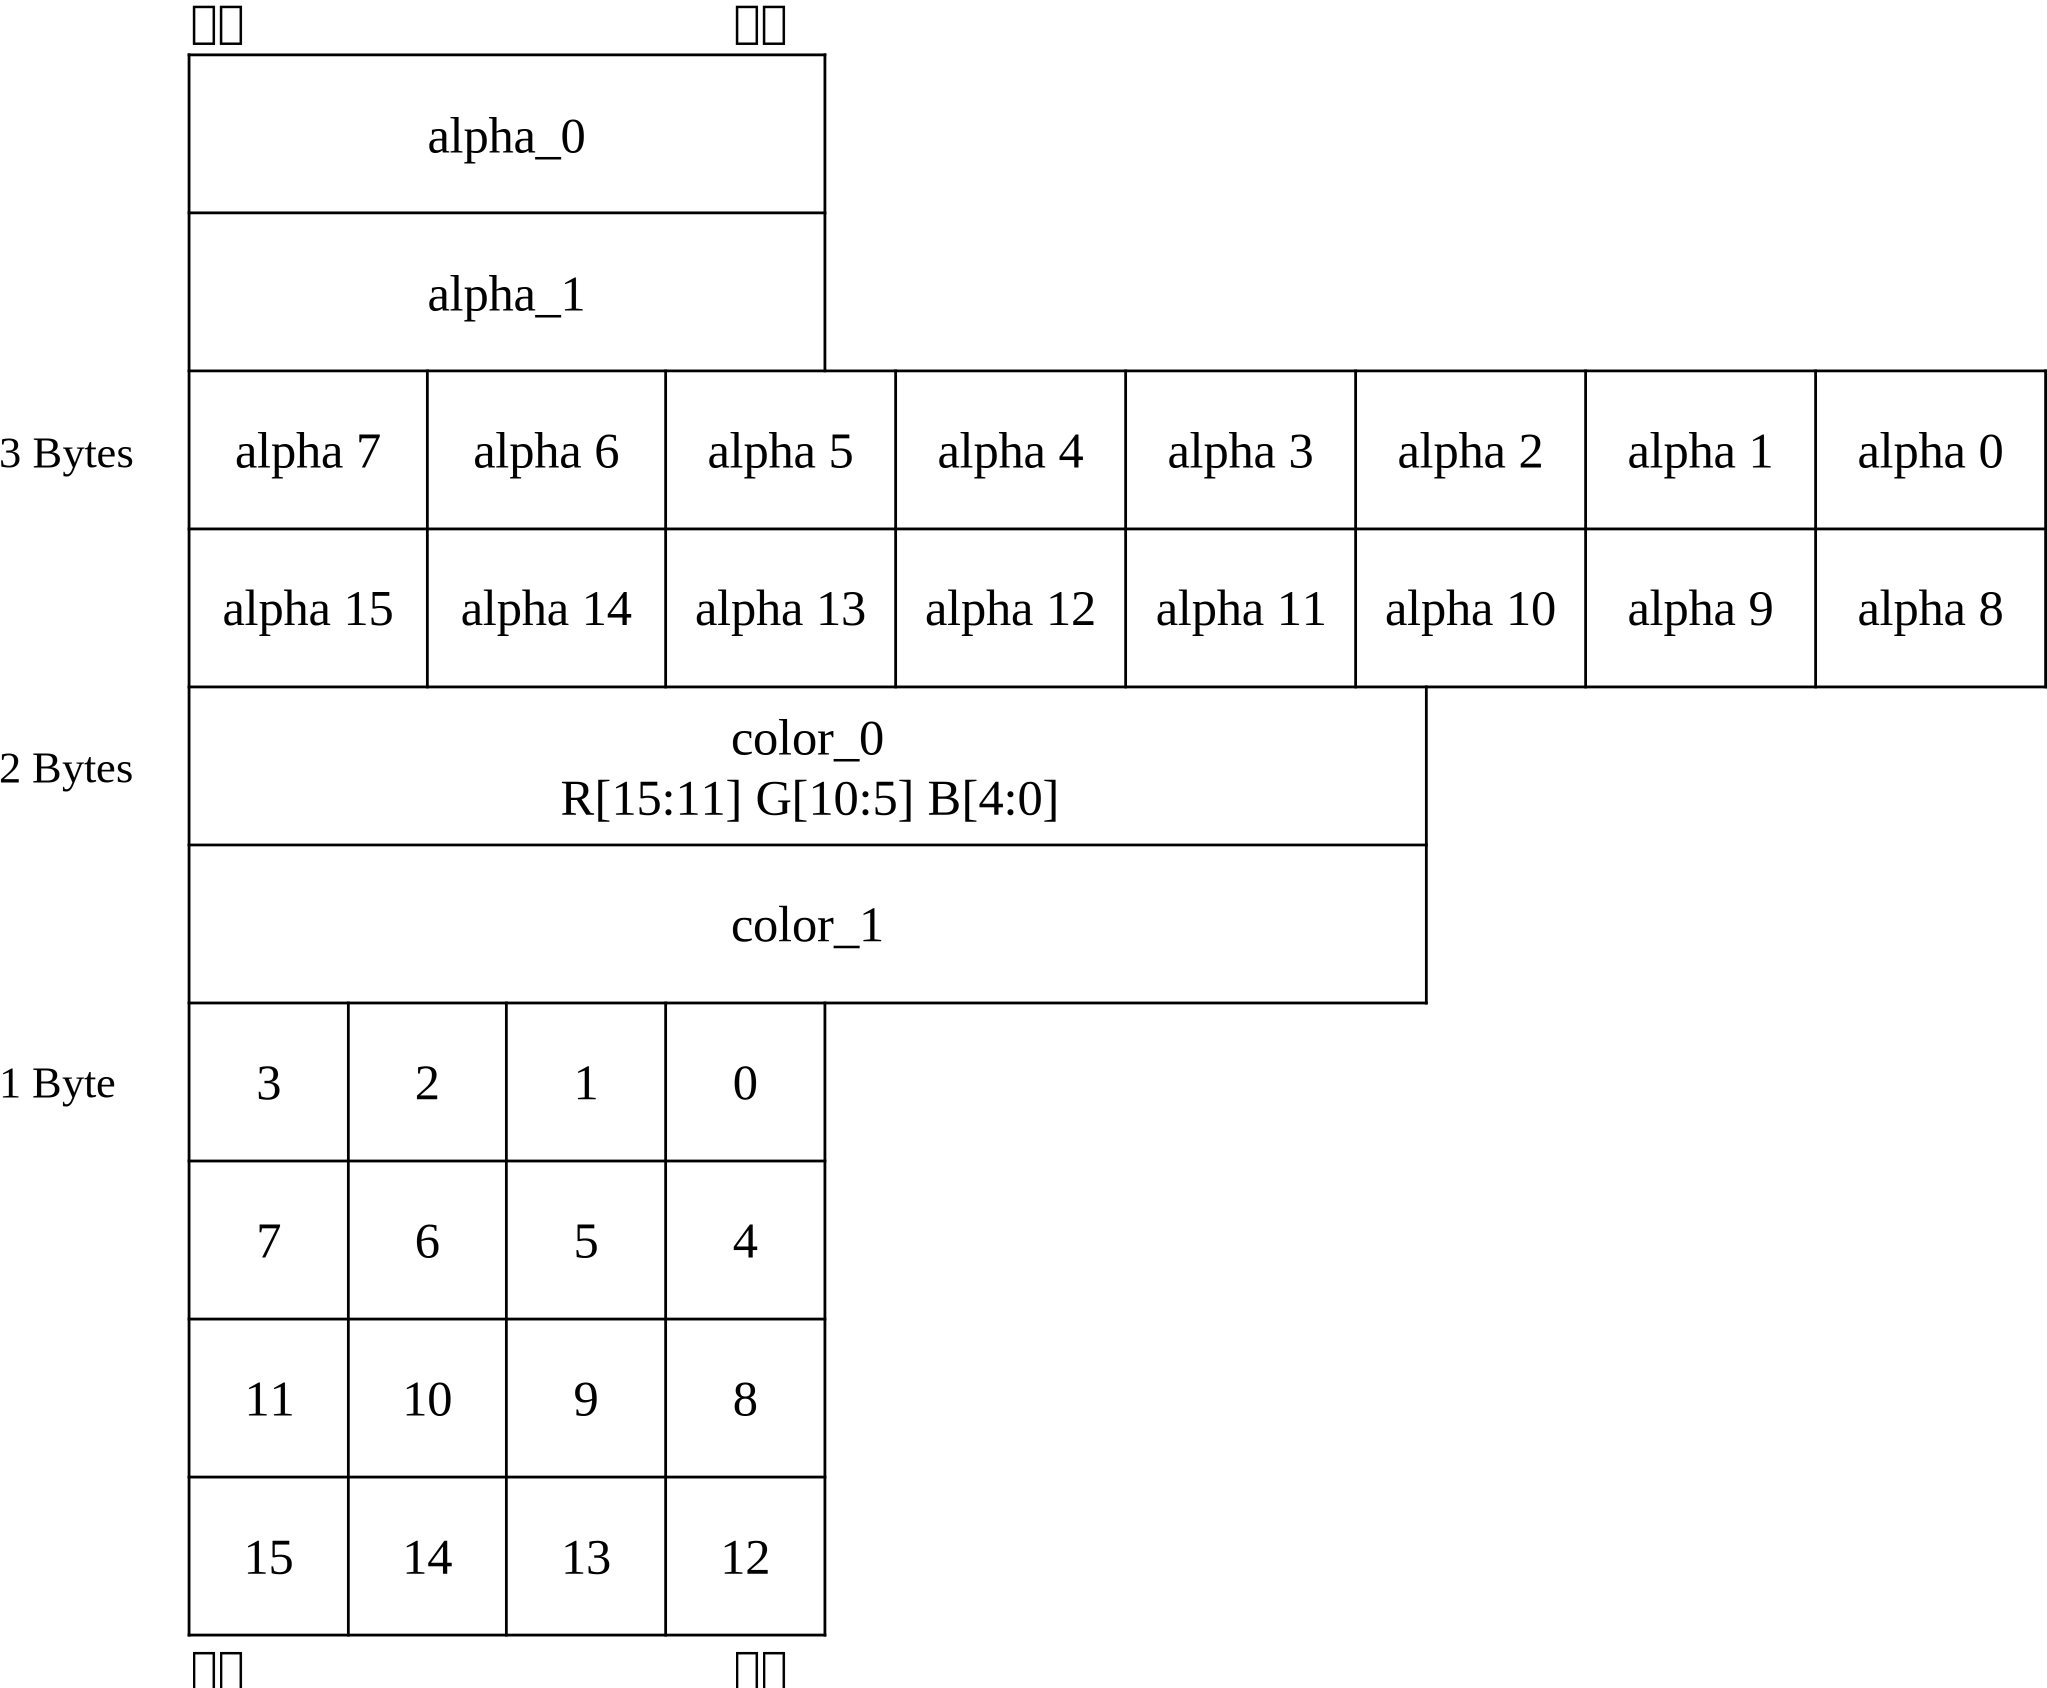
\includegraphics[width=0.7\textwidth]{figures/BC3.png}
    \caption{BC3格式中每个块的数据布局\cite{BC1-5}}
    \label{fig:BC3}
\end{figure}

BC4格式用于存储单通道的颜色数据,如图\ref{fig:BC4}所示,BC4存储两个8位颜色端点与16个3位的权重,
解压时同样通过线性插值恢复颜色数据。
最终每个4x4纹素块存储为8字节,相较于压缩前的每纹素8位的单通道纹理共16字节达到了2:1的压缩比。

\begin{figure}[htbp]
    \centering
    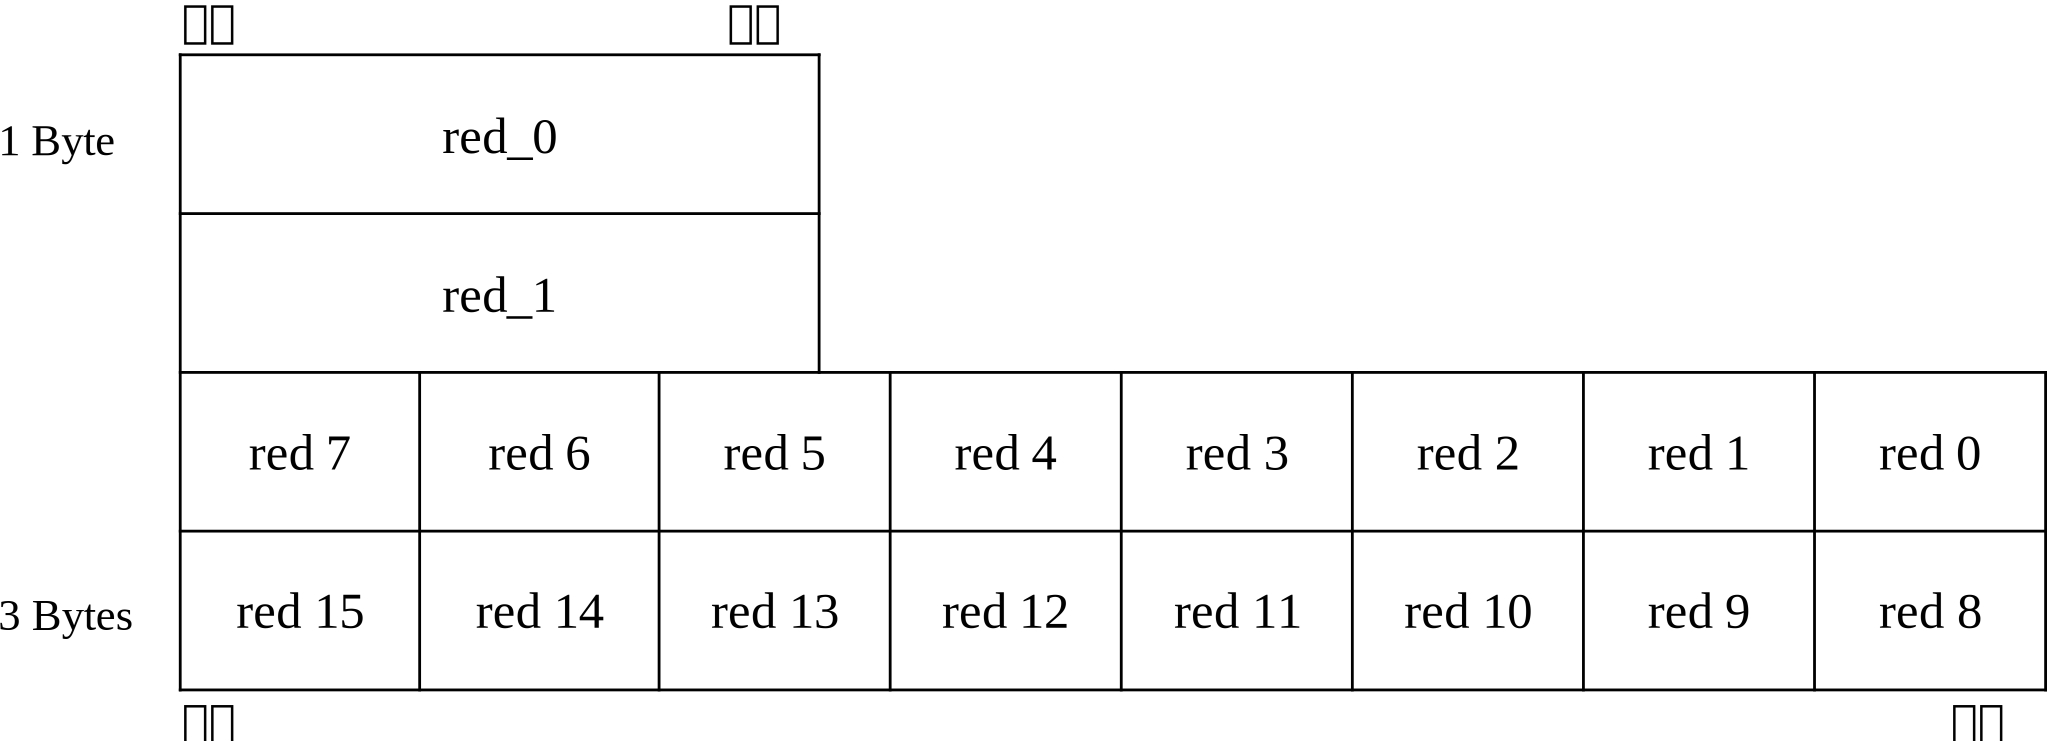
\includegraphics[width=1\textwidth]{figures/BC4.png}
    \caption{BC4格式中每个块的数据布局\cite{BC1-5}}
    \label{fig:BC4}
\end{figure}

BC5格式用于存储双通道的颜色数据,可以视为双通道版本的BC4格式。如图\ref{fig:BC5}所示,BC5对每个通道分别存储两个8位颜色端点与16个3位的权重,
解压时需要在每个通道分别进行线性插值恢复颜色数据。
最终每个4x4纹素块存储为16字节,相较于压缩前的每纹素16位的双通道纹理共32字节达到了2:1的压缩比。

\begin{figure}[htbp]
    \centering
    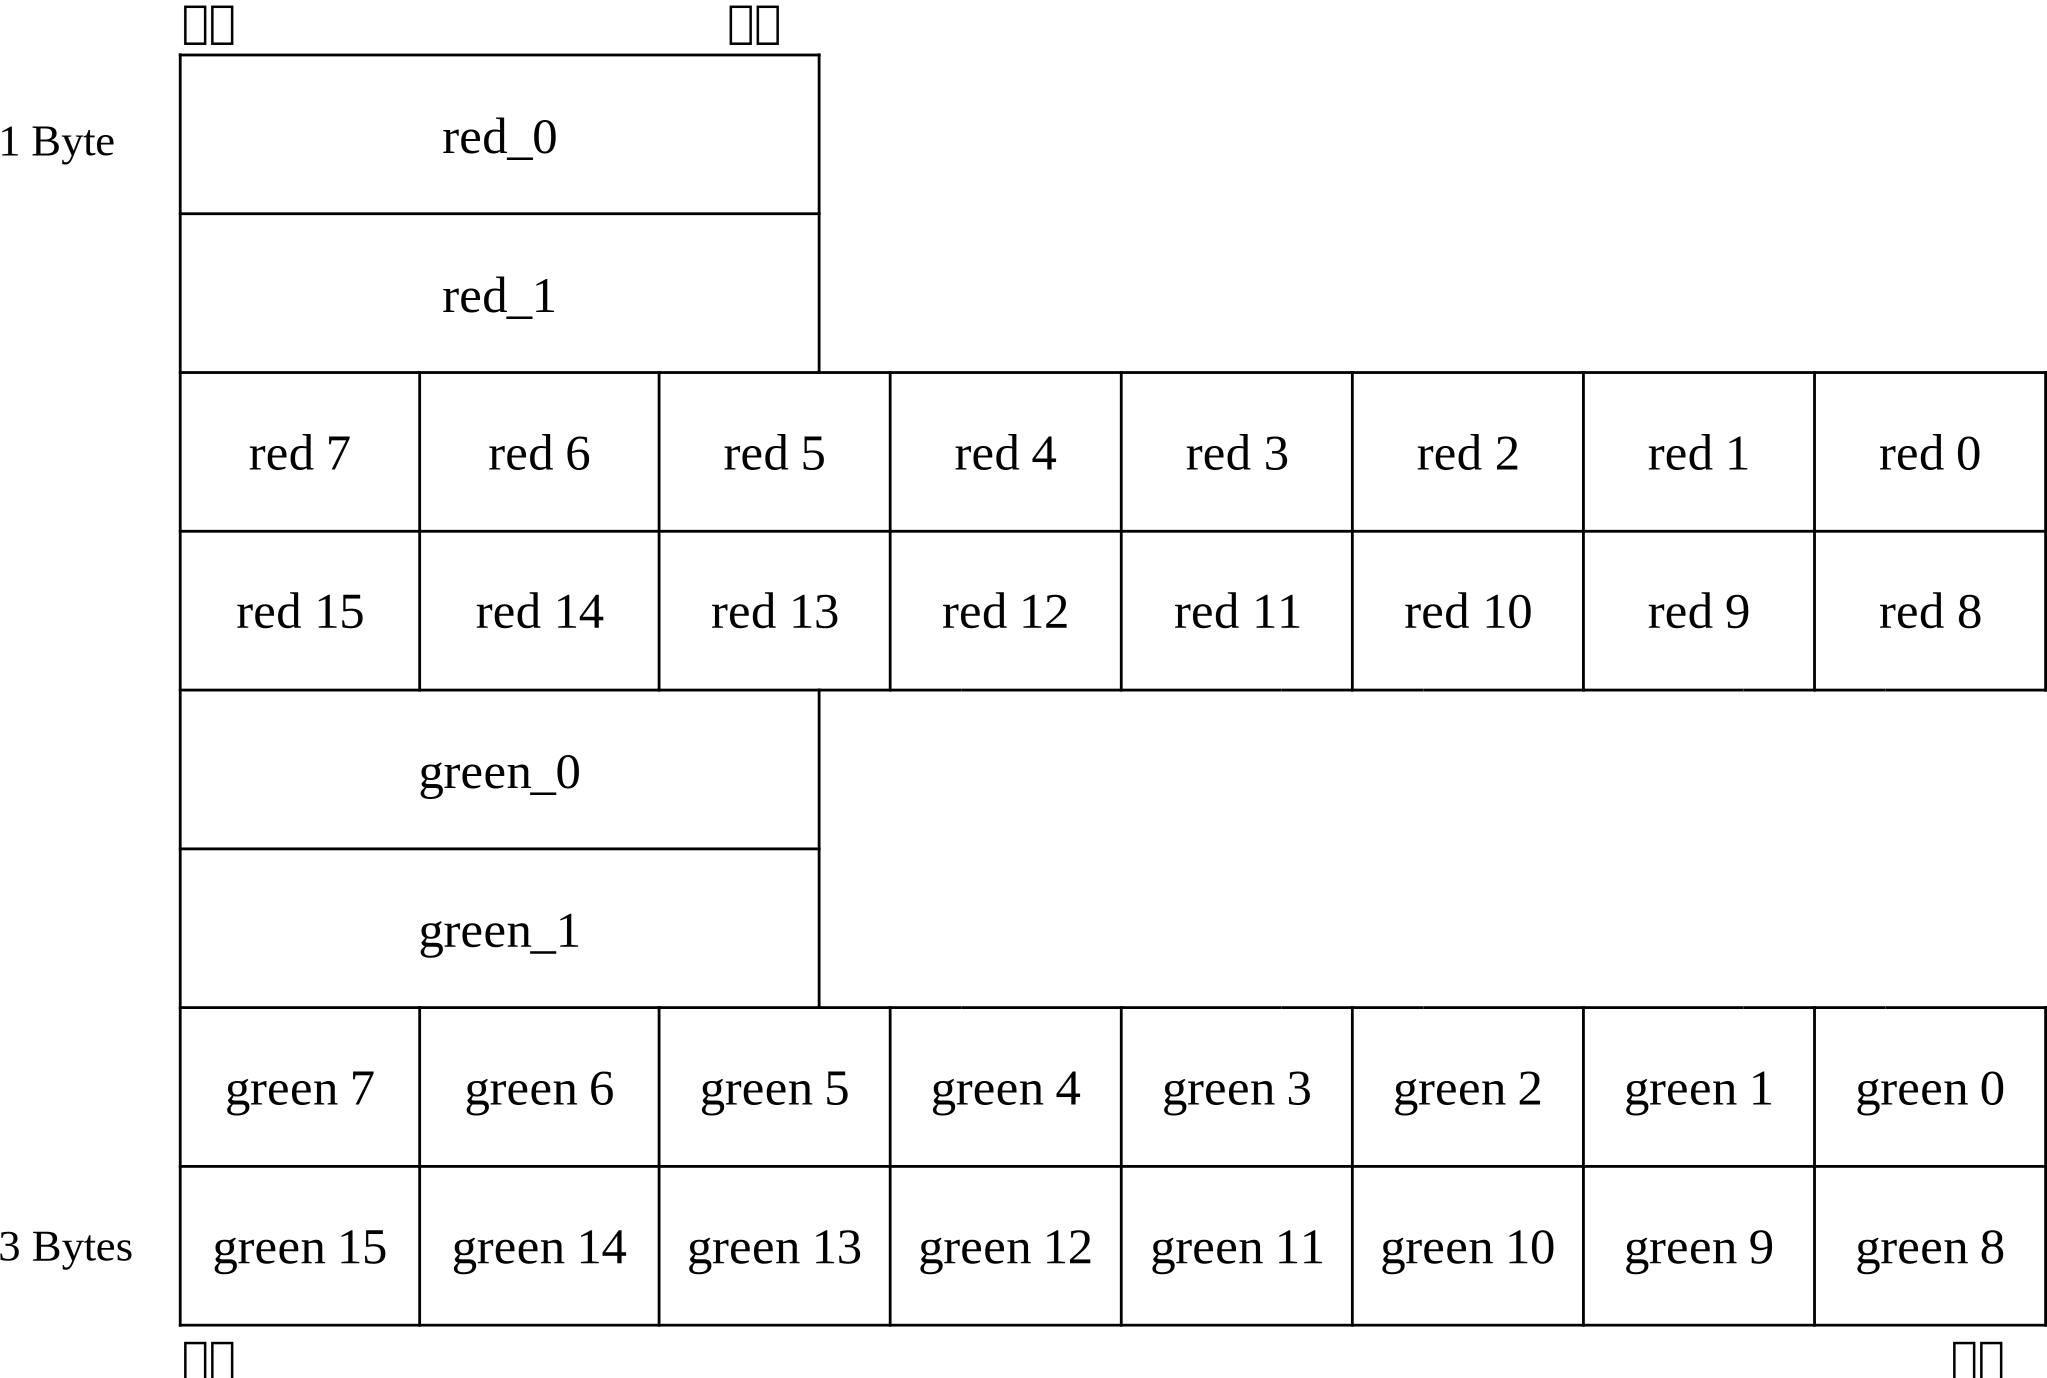
\includegraphics[width=1\textwidth]{figures/BC5.png}
    \caption{BC5格式中每个块的数据布局\cite{BC1-5}}
    \label{fig:BC5}
\end{figure}

总体上BC2至BC5这4种格式都是在BC1基础上的改进,整体上的压缩思想都是将每4x4纹理块中的16个颜色值压缩为2个颜色端点与16个权重,
解压时根据权重对颜色端点进行线性插值。

\subsection{BC6纹理格式}

BC6格式被专门设计用于高动态范围(HDR)的RGB纹理,每4x4块使用16字节存储。与BC1至BC5类似,BC6格式同样会将颜色压缩为颜色端点与权重,
不同之处在于BC6引入了分区、模式等概念以及BC6具有独特的量化方式。BC6H的每个4x4块由模式位、颜色端点、颜色权重和分区索引组成。

分区是指将4x4的块分割为多个独立的子块单独压缩,
如图\ref{fig:2-Partition}所示,4x4的纹理块被分为红色与绿色两个分区,每个分区具有独立的颜色端点与权重。
BC6共包括32种不同的分区,编码时编码器会根据压缩误差选择最合适的分区进行编码。

\begin{figure}[htbp]
    \centering
    \includegraphics[width=1\textwidth]{figures/2-Partition.pdf}
    \caption{BC6格式的双分区布局\cite{ASTC}}
    \label{fig:2-Partition}
\end{figure}

模式是指压缩每4x4块时使用的编码配置,每种编码配置包括分区数量、颜色位数、权重位数以及端点格式等压缩方式。
BC6共有14种不同的模式,如表\ref{tab:BC6Mode}所示,其中模式1至模式10为双分区、模式11至模式14为单分区,
对于双分区模式,会有5位的分区索引作为每个分区的唯一标识。
每种模式还具有不同的颜色端点位数以及权重位数,例如模式10使用每通道6位(双分区共72位)的颜色端点和3位(双分区共48位)的权重进行存储。
由于每个4x4块可以使用不同的模式,还有专门的模式位作为每个模式的唯一标识。
实际编码时,对于每4x4的像素块,编码器都会根据编码产生的压缩误差在众多模式中选择最佳的编码配置。

\begin{table}[htbp]
    \centering
    \caption{BC6格式中每个纹理块的14种模式\cite{BC6H}}
    \label{tab:BC6Mode}        
    % \resizebox{6cm}{!}{
    \begin{tabular}{ccccc}
    \toprule
    模式 & 权重总位数(bits) & 分区标识位 & 颜色端点总位数(bits) & 模式标识位\\
    \midrule
    1   &   46    &  5  &   75  &   2(00)   \\
    2   &   46    &  5  &   75  &   2(01)   \\
    3   &   46    &  5  &   72  &   5(00010)   \\
    4   &   46    &  5  &   72  &   5(00110)   \\
    5   &   46    &  5  &   72  &   5(01010)   \\
    6   &   46    &  5  &   72  &   5(01110)   \\
    7   &   46    &  5  &   72  &   5(10010)   \\
    8   &   46    &  5  &   72  &   5(10110)   \\
    9   &   46    &  5  &   72  &   5(11010)   \\
    10  &   46    &  5  &   72  &   5(11110)   \\
    11  &   63    &  0  &   60  &   5(00011)   \\
    12  &   63    &  0  &   60  &   5(00111)   \\
    13  &   63    &  0  &   60  &   5(01011)   \\
    14  &   63    &  0  &   60  &   5(01111)   \\
    \bottomrule
    \end{tabular}
    % }   
\end{table}

BC6的量化过程比较特殊,权重部分的量化与DXT格式中的其他子格式相同,使用均匀量化。
但对于颜色端点使用了非均匀量化,首先会将原始的16位浮点值按照内存中实际存储的二进制值,
解读为16位整数值,再进行均匀量化:
\begin{equation}
    Q(r)=\left \lfloor \frac{\text{F16toInt16}(r)}{\text{Int16\_Max}} \times (2^{b}-1) \right \rceil
\end{equation}
其中$r$表示量化前的16位浮点值,F16toInt16(r)表示
将16位浮点值$r$按照内存中实际存储的二进制值解读为16位整数值,
Int16\_Max表示Int16所能表示的最大值,
$b$表示量化位数,$Q(r)$表示量化后的整数值,
$\lfloor \cdot \rceil$表示四舍五入函数。

解量化时首先对颜色端点解量化,然后将16位插值结果按照内存中实际存储的二进制值解读为16位浮点值,
解量化函数为:
\begin{equation}\label{eqn-6}
    Q'(q)=\text{Int16toF16}(\frac{q}{2^{b}-1}*\text{Int16\_Max})
\end{equation}
其中$q$表示量化后的整数值,$b$表示量化位数,Int16\_Max表示Int16所能表示的最大值,
Int16toF16表示
将16位整数值按照内存中实际存储的二进制值解读为16位浮点值,
$Q'(q)$表示解量化得到的16位浮点值。



\subsection{BC7纹理格式}

BC7格式是DXT中最复杂的纹理格式,包含了BC1至BC5格式具有的所有特点,
用于对 RGB 和 RGBA 纹理进行高质量压缩,
每4x4块使用 16 字节存储。与BC6类似,BC7也具有分区与模式的概念,除此之外BC7还引入了旋转。
旋转是指压缩前先将A通道与RGB通道的某一个进行交换,旋转包括RGBA、AGBR、RABG、RGAB四种,
例如AGBR表示将R通道与A通道进行交换,这样做的目的是可以将某一个通道使用更多位数进行存储,
从而提高该通道的压缩质量。

BC7共具有8种不同的模式,如表\ref{tab:BC7Mode}所示,
其中模式0至模式3用于压缩RGB纹理,模式4至模式7用于压缩RGBA纹理。
模式0至模式3与BC1类似,仅增加了多分区,其中模式0与模式2为三分区,模式1和3为双分区。
模式4与模式5将RGB通道与A通道分开压缩,类似BC3,但增加了旋转操作,可以将RGB中的某个通道与A通道交换,
由于A通道具有单独的颜色端点与权重,因此可以获得更好的压缩质量。模式4还具有2种不同的权重位数设置,
即对RGB通道使用2位权重,A通道使用3位权重;或者RGB通道使用3位权重,A通道使用2位权重。
因此模式4具有8种配置(4种旋转*2种权重设置)、模式5具有4种配置(4种旋转)。
模式6存储两个RGBA颜色端点与权重,类似BC1。模式7为双分区模式,
每个分区类似模式6,共具有64种不同分区。

\begin{table}[htbp]
    \centering
    \caption{BC7格式中每个纹理块的8种模式\cite{BC7}}
    \label{tab:BC7Mode}        
    % \resizebox{6cm}{!}{
    \begin{tabular}{ccccc}
    \toprule
    模式 & 权重总位数(bits) & 分区标识位 & 颜色端点总位数(bits) & 模式标识位\\
    \midrule
    0   &   45    &  4  &   78  &   1(1)   \\
    1   &   46    &  6  &   74  &   2(01)   \\
    2   &   29    &  6  &   90  &   3(001)   \\
    3   &   30    &  6  &   88  &   4(0001)   \\
    4   &   31/47(RGB/A)    &  42  &   72  &   5(00001)   \\
    5   &   31/31(RGB/A)    &  58  &   72  &   6(000001)   \\
    6   &   63    &  5  &   58  &   7(0000001)   \\
    7   &   30    &  5  &   84  &   8(00000001)   \\
    \bottomrule
    \end{tabular}
    % }   
\end{table}


\section{混合专家模型}

混合专家模型(Mixture of Experts,MoE)最早由 Jacobs 等\cite{jacobs1991adaptive}提出,
如图\ref{fig:MoE}所示,MoE通过结合多个不同的专家网络和一个门控网络来决定哪些专家应参与计算,从而有效减少训练数据中不同子任务之间的干扰,
进而提升模型的学习速度和泛化能力。在 MoE 中,每个专家需生成完整的输出向量,而非对各专家的输出进行线性混合。
这一特性与纹理压缩中的编码过程相符,
即从多种不同的编码模式中选择最佳模式,
而非将多种编码模式进行混合。

\begin{figure}[htbp]
    \centering
    \includegraphics[width=1\textwidth]{figures/moe.pdf}
    \caption{最早的混合专家模型\cite{jacobs1991adaptive}}
    \label{fig:MoE}
\end{figure}

自 MoE 架构提出以来,它已被广泛应用于多种机器学习模型中,包括支持向量机\cite{collobert2002parallel}、
混合高斯过程模型\cite{tresp2001mixtures,rasmussen2001infinite}
以及神经网络\cite{aljundi2017expert,garmash2016ensemble,eigen2013learning}。

然而,MoE 架构在条件计算中需要频繁进行分支操作以决定激活哪些专家网络,这与 GPU 的高度并行计算架构并不匹配,
导致计算效率难以提升,训练成本显著增加,从而限制了 MoE 架构在大规模网络中的应用。
为了解决这一问题,Shazeer 等\cite{shazeer2017outrageously}为 MoE 架构的门控网络引入了 softmax 和 Noisy Top-K 方法,
从而克服了 MoE 的分支问题,并在模型容量上实现了超过 1000 倍的提升。

目前,MoE 架构已广泛应用于 Transformers\cite{vaswani2017attention}中,
例如 Switch Transformer\cite{fedus2022switch}、
GLaM\cite{du2022glam}、ST-MOE\cite{zoph2022st}
和 GShard\cite{lepikhin2020gshard}等。


最近,DeepSeek-V3\cite{liu2024deepseek}作为一种先进的专家混合语言模型,
采用了DeepSeekMoE架构\cite{dai2024deepseekmoe}以实现高效推理和经济训练。
传统的 Top-K MoE 架构通过亲和力得分激活 N 个专家中的前 K 个,
但这种方法存在知识混合性(Knowledge Hybridity)和知识冗余(Knowledge Redundancy)两个潜在问题。
为了解决这些问题,如图\ref{fig:DeepSeekMoE}所示,DeepSeekMoE 架构基于两个主要策略进行了改进:(1)细粒度专家分割,
将专家细分为 m×N 个,并从中激活 m×K 个,以实现更灵活的专家组合;(2)共享专家隔离,
将某些专家隔离为共享专家,这些专家始终处于激活状态,旨在捕获和巩固不同背景下的共同知识。
受到 DeepSeekMoE 架构的启发,本文为可微块压缩模型引入了一种基于MoE架构的分区配置选择器,以提高分区配置选择的计算效率。

\begin{figure}[htbp]
    \centering
    \includegraphics[width=1\textwidth]{figures/DeepSeekMoE.png}
    \caption{DeepSeekMoE与传统MoE\cite{dai2024deepseekmoe}}
    \label{fig:DeepSeekMoE}
\end{figure}

\section{神经压缩}

神经压缩是指使用神经网络压缩某种材质的纹理集的技术。
这类技术通常使用特征网格表示纹理,运行时根据纹理像素的坐标,在特征网格上采样特征向量,
然后通过神经网络对特征向量进行解码。
NTC\cite{vaidyanathan2023random}的神经压缩框架如图\ref{fig:Nvidia}所示。
某种材质的纹理集(包括漫反射纹理、法线纹理、ARM纹理等)通过多分辨率的特征网格进行表示。
训练时,对于训练样本的某个纹理坐标,首先在特征网格中采样出特征向量,经过模拟量化后
通过神经网络进行解码。这种方法的优点在于可以同时压缩多通道的纹理数据,例如可以同时压缩将
3通道漫反射纹理、2通道法线纹理、3通道ARM纹理拼接成的8通道纹理,而传统的纹理块压缩技术最高仅支持4通道纹理。
更高的压缩通道数提供了更高的压缩率,同时减少了纹理采样次数。
在相同空间下,这种方法获得了更高的压缩质量,不足之处在于采样后需要进行网络推理,增加了额外的GPU开销。

\begin{figure}[htbp]
    \centering
    \includegraphics[width=1\textwidth]{figures/Nvidia.png}
    \caption{NTC的神经压缩框架\cite{vaidyanathan2023random}}
    \label{fig:Nvidia}
\end{figure}

BCf\cite{weinreich2024real}的神经压缩框架如图\ref{fig:BCf}所示,其中特征网格以BC6格式存储,并通过可微的BC6解码器对特征
网格进行训练。运行时从BC6格式的特征网格中采样特征向量并进行网络推理。这种方法进一步提高了
纹理集的压缩率。
不足之处在于仅解码器的优化架构无法根据编码产生的压缩误差选择最佳编码配置,只能以固定配置进行优化,
一定程度限制了BC6的压缩能力。

\begin{figure}[htbp]
    \centering
    \includegraphics[width=1\textwidth]{figures/BCf.png}
    \caption{BCf的神经压缩框架\cite{weinreich2024real}}
    \label{fig:BCf}
\end{figure}


\section{基于移动基分解的光照数据压缩}

为了追求高质量渲染效果,全局光照技术在游戏中被广泛应用,由于GPU硬件限制,实时光线追踪
对于大多数设备难以以较高帧率运行,因此预计算的照明技术依然是最常用的光照解决方案。
然而对于大规模场景,仅以球谐函数形式存储的体积辐射度将占用GB级别的显存\cite{silvennoinen2021moving},
对于许多平台,这将占用大多数的显存空间,几乎没有足够的剩余空间分配给几何与纹理数据。
为解决这一问题,Silvennoinen与Sloancite\cite{silvennoinen2021moving}提出了移动基分解方法(Moving Basis Decomposition,MBD),
这种方法将空间中的光照数据分解为一系列基向量与系数进行压缩存储,运行时通过空间滤波解压光照数据。

为了压缩存储预计算的光照数据,MBD 方法将光照数据在空间域分解为一系列基向量$b$与系数$c$,重建函数 $\hat{f}:R^3\to R^D$ 如下:
\begin{equation}
\hat f(x)=\sum_{l}^L c_{l} (x)b_{l}(x)
\end{equation}
其中 $\hat{f}(x)$ 表示在位置 $x$ 处的重建光照值,$L$ 表示 MBD 的秩,$c_l(x)$ 和 $b_l(x)$ 表示第 $l$ 个系数和基向量,它们的具体表达式如下:
\begin{equation}
c_{l}(x)=\sum_{m}\phi_{m} (x)c_{m,l}
\end{equation}
\begin{equation}
b_{l}(x)=\sum_{n}\psi_{n} (x)B_{n,l}
\end{equation}
其中 $\phi_{m}: R^{3} \rightarrow R$与$\psi_{n}: R^{3} \rightarrow R$分别表示系数与基向量的核函数,例如三线性插值。 $c_{m,l}$表示第 $l$ 在核函数 $\phi_m$ 上的系数,$B_{n,l}$ 表示第 $l$ 个在核函数 $\psi_n$ 上的基向量。

MBD\cite{silvennoinen2021moving} 算法首先利用 PCA 方法初始化系数与基向量,然后通过随机梯度下降、线搜索回溯等优化方法调整系数与基向量,以最小化重建误差。
相较于其他基于PCA的降维方法,例如BPCA\cite{nishino2005clustered}、CPCA\cite{sloan2003clustered}等,MBD\cite{silvennoinen2021moving}提供了更好的压缩质量,实现了几乎无缝的重建效果。

\section{HDR纹理的RGBM编码}

传统的LDR(Low Dynamic Range)纹理通常使用每通道8位无符号整数存储颜色值,颜色范围为0-255。
HDR(High Dynamic Range)纹理使用16位或32位浮点数存储颜色值,
能够表示更广泛的亮度范围,从而避免过暗或过亮区域细节的丢失。
目前桌面端的Windows系统上通常使用DXT格式中的BC6格式压缩HDR纹理,
BC6格式跟随Direct3D 11被引入Windows系统,Direct3D 11出现前Windows系统
上仅有支持LDR纹理的BC1至BC5格式,因此出现了RGBM编码技术,通过将RGB三通道的HDR纹理
转换为RGBA四通道的LDR纹理,从而使得HDR纹理可以使用LDR纹理格式进行压缩。

RGBM编解码的流程分别采用算法\ref{algo:RGBMEncode}与算法\ref{algo:RGBMDecode}进行,
整体思想是利用A通道存储缩放因子,从而实现HDR到LDR的缩放。

\begin{algorithm}
    \caption{RGBM编码}
    \label{algo:RGBMEncode}
    \SetKwFunction{FMain}{RGBMEncode}
    \SetKwProg{Fn}{Function}{:}{}
    \SetKw{FInt}{int4}
    \SetKw{Ffloat}{float4}
    \SetKw{Tfloat}{float3}
    \SetKw{float}{float}
    \SetKw{clamp}{clamp}
    \SetKw{max}{max}
    \SetKw{min}{min}
    \SetKw{sqrt}{sqrt}
    \SetKw{round}{round}    
    \SetKw{ceil}{ceil}   
    \KwIn{HDR\_color(原始HDR纹理中的每个RGB纹素), Multiplier(RGBM编码支持的最大值)}
    \KwOut{LDR\_color(编码后LDR纹理中的每个RGBA纹素)}
    \Fn{\FMain{\Tfloat HDR\_color, \float  Multiplier}}
    {
        \Tfloat RGB = HDR\_color / Multiplier\;
        \float MaxRGB = \max(RGB.r, RGB.g, RGB.b)\;
        \float SqrtMaxRGB = \sqrt(MaxRGB)\;
        \float SqrtMScale = \min(1, \ceil(SqrtMaxRGB * 255) / 255)\;
        \float MScale = SqrtMScale * SqrtMScale\;
        \float Ratio = \min(1, MScale / MaxRGB)\;
        \Tfloat RGBScale = RGB * Ratio / MScale\;
        RGBScale = \round(RGBScale * 255) / 255\;
        \FInt LDR\_color = \clamp(\FInt(RGBScale * 255, SqrtMScale * 255),0,255)\;
        \Return LDR\_color\;
    }
\end{algorithm}
\begin{algorithm}
    \caption{RGBM解码}
    \label{algo:RGBMDecode}
    \SetKwFunction{FMain}{RGBMDecode}
    \SetKwProg{Fn}{Function}{:}{}
    \SetKw{FInt}{int4}
    \SetKw{Ffloat}{float4}
    \SetKw{Tfloat}{float3}
    \SetKw{float}{float}
    \SetKw{clamp}{clamp}
    \SetKw{max}{max}
    \SetKw{min}{min}
    \SetKw{sqrt}{sqrt}
    \SetKw{round}{round}    
    \SetKw{ceil}{ceil}   
    \KwIn{LDR\_color(编码后LDR纹理中的每个RGBA纹素), Multiplier(RGBM编码支持的最大值)}
    \KwOut{HDR\_color(原始HDR纹理中的每个RGB纹素)}
    \Fn{\FMain{\FInt LDR\_color, \float  Multiplier}}
    {
        \Ffloat fLDR\_color = LDR\_color / 255\;
        \Tfloat HDR\_color = fLDR\_color.rgb*fLDR\_color.a*fLDR\_color.a*Multiplier\;
        \Return HDR\_color\;
    }
\end{algorithm}
% \begin{algorithm}
%     \caption{HDR纹理的RGBM编解码}
%     \label{algo:RGBM Encode}
%     \SetAlgoLined
%     \SetKwFunction{RGBMEncode}{RGBMDecode}

%     initialization\;
%     \While{not at end of this document}{
%       read current\;
%       \eIf{understand}{
%         go to next section\;
%         current section becomes this one\;
%       }{
%         go back to the beginning of current section\;
%       }
%     }
    
%     \Fn{\RGBMEncode{num\_cycles}}{
%         执行图像内存屏障、布局转换并重置时间戳查询池\;
%         等待先前命令完成\;
%         cmdBuf \gets 从池中分配命令缓冲区()\;
%         在 cmdBuf 中录制写时间戳 $ts_1$ 命令\;
%         \For{i \gets 1 \textbf{to} num\_cycles}{
%             在 cmdBuf 中录制绑定图形管线和描述符命令\;
%             在 cmdBuf 中录制绘制命令\;
%         }
%         在 cmdBuf 中录制写时间戳 $ts_2$ 命令\;
%         提交至命令队列\;
%         等待先前命令完成\;
%         \Return $(ts_2 - ts_1) \times unitTs$\;
%     }

%   \end{algorithm}

\section{本章小结}

本章对相关工作进行了简要的介绍。首先介绍了DXT纹理格式,包括BC1至BC7这7种纹理块压缩格式的具体内容。
然后介绍了混合专家模型的发展脉络。最后介绍了后续实验中采用的三个应用场景:
神经压缩、基于移动基分解的光照数据压缩以及HDR纹理的RGBM编码。
值得注意的是,虽然现有工作已经对可微BC6解码器有了比较深入的研究,
但是由于仅解码器的框架的局限性,固定编码配置导致纹理块压缩格式的编码能力没有被充分利用,
因此支持编码配置选择从而获得更高压缩质量的可微编解码器框架是值得研究的方向。
